%%%%%%%%%%%%%%%%%%%%%%%%%%%%%%%%%%%%%%%%%%%%%%%%%%%%%%%%%%%%%%%%%%%%%%
% How to use writeLaTeX: 
%
% You edit the source code here on the left, and the preview on the
% right shows you the result within a few seconds.
%
% Bookmark this page and share the URL with your co-authors. They can
% edit at the same time!
%
% You can upload figures, bibliographies, custom classes and
% styles using the files menu.
%
%%%%%%%%%%%%%%%%%%%%%%%%%%%%%%%%%%%%%%%%%%%%%%%%%%%%%%%%%%%%%%%%%%%%%%

\documentclass[12pt]{article}
\usepackage{adjustbox}
\usepackage{sbc-template}
\usepackage{todonotes}
\usepackage{graphicx,url}
\usepackage{amsmath}
\usepackage{multirow}
\usepackage[utf8]{inputenc}  
\usepackage[T1]{fontenc}
\usepackage{xspace}
\usepackage{url}
\usepackage{graphicx}
\usepackage{subfig}
\usepackage{unicode-math}
\usepackage[T1]{fontenc}
\usepackage{xspace}
\usepackage{url}
\usepackage[brazil]{babel}

\sloppy

\title{Calculo Numérico\\Trabalho\_1}


\author{Prof. Dra. Larissa de Freitas \inst{1},\\Guilherme de Souza\inst{1}}

\begin{document} 

\maketitle
%\br
\section{Funções}
\begin{eqnarray}
$\lambda x: 5x^{3} - 2x^{2} + 8x - 10$\\
$\lambda x: 2x^{3} + 5x^{2} + \sin x - 30$\\
$\lambda x: e^{-x2}\cos x$\\
    $\lambda x: (x+1)(x-1)(x-3)^{5}\\
    $\lambda x: (x+2)^{3}\sqrt{x^{2}+1}$
\end{eqnarray}

\section{Resultados}
%\begin{table}[]
%\begin{tabular}{lllll}
%\multicolumn{5}{c}{\textbf{Função um}}                                                                                                                                                           \\ \hline
%\multicolumn{1}{l|}{\textbf{Metodos}}         & \multicolumn{1}{l|}{Bisseção}           & \multicolumn{1}{l|}{Falsa Posição}      & \multicolumn{1}{l|}{Secante}            & Tangente           \\ \hline
%\multicolumn{1}{l|}{\textbf{Raiz Aproximada}} & \multicolumn{1}{l|}{0.9453692918468732} & \multicolumn{1}{l|}{0.9453692918429207} & \multicolumn{1}{l|}{0.9453692918467353} & 0.9453692918280763 \\ \hline
%\multicolumn{1}{l|}{\textbf{Iterações}}       & \multicolumn{1}{l|}{35}                 & \multicolumn{1}{l|}{51}                 & \multicolumn{1}{l|}{8}                  & 15
%\end{tabular}
%\end{table}

Na tabela 1, podemos analisar os resultados encontrados, pode-se ver que a diferença entre as raízes somente é notada a partir da decima segunda casa decimal. Já em número de operações, ou seja, iterações os dois ultimos métodos se sairam melhor, encontrando as raízes em somente oito e quinze iterações.

\begin{table}[!h]
\begin{center}
\begin{tabular}{lll}
\multicolumn{3}{c}{\textbf{Função Um}}                                                                              \\ \hline
\multicolumn{1}{l|}{\textbf{Métodos}}       & \multicolumn{1}{l|}{\textbf{Raízes Aproximadas}} & \textbf{Iterações} \\ \hline
\multicolumn{1}{l|}{\textbf{Bisseção}}      & \multicolumn{1}{l|}{0.9453692918468732}          & 35                 \\ \hline
\multicolumn{1}{l|}{\textbf{Falsa Posição}} & \multicolumn{1}{l|}{0.9453692918429207}          & 51                 \\ \hline
\multicolumn{1}{l|}{\textbf{Secante}}       & \multicolumn{1}{l|}{0.9453692918467353}          & 8                  \\ \hline
\multicolumn{1}{l|}{\textbf{Tangente}}      & \multicolumn{1}{l|}{0.9453692918280763}          & 15                
\end{tabular}
    \caption{Raízes aproximadas e número de interações da função um aplicada aos quatro métodos.}
\end{center}
\end{table}

Dando continuidade, o mesmo pode-se observar na Tabela 2, que se assemelha a 1. As raízes encontradas, novamente só sofrem alterações a partir da decima segunda casa decimal. Desta vez realizando menos Iterações do que a função anterior, porém, mantendo a mesma ordem de crescimento quanto ao número de iterações.

\begin{table}[!h]
\begin{center}
\begin{tabular}{lll}
\multicolumn{3}{c}{\textbf{Função Dois}}                                                                            \\ \hline
\multicolumn{1}{l|}{\textbf{Métodos}}       & \multicolumn{1}{l|}{\textbf{Raízes Aproximadas}} & \textbf{Iterações} \\ \hline
\multicolumn{1}{l|}{\textbf{Bisseção}}      & \multicolumn{1}{l|}{1.8797824746652623}          & 36                 \\ \hline
\multicolumn{1}{l|}{\textbf{Falsa Posição}} & \multicolumn{1}{l|}{1.8797824746628244}          & 44                 \\ \hline
\multicolumn{1}{l|}{\textbf{Secante}}       & \multicolumn{1}{l|}{1.8797824746647178}          & 8                  \\ \hline
\multicolumn{1}{l|}{\textbf{Tangente}}      & \multicolumn{1}{l|}{1.879782474667825}           & 9
\end{tabular}
\end{center}
    \caption{Raízes aproximadas e número de interações da função dois aplicada aos quatro métodos.}
\end{table}

De acordo com a Tabela 3, podemos notar uma diferença mais gritante. As raízes semelhantes, elas sofrem alterações a partir da oitava casa decimal e ainda, no método da secante podemos ver uma raíz com valor bem inferior, variando $\pm$ 0.4 quanto aos outros métodos. Quanto a interações, a secante chegou a concluir em somente 5 iterações, enquanto a tangente levou 500. Com isso podemos ver uma mudança de cenário, os dois primeiros métodos, passaram a fazer menos iterações quando comparado a tangente, porém, a secante ainda realiza menos, mas como efeito, aparentemente possui uma menos precição.
\begin{table}[!h]
\begin{center}
\begin{tabular}{lll}
\multicolumn{3}{c}{\textbf{Função Três}}                                                                            \\ \hline
\multicolumn{1}{l|}{\textbf{Métodos}}       & \multicolumn{1}{l|}{\textbf{Raízes Aproximadas}} & \textbf{Iterações} \\ \hline
\multicolumn{1}{l|}{\textbf{Bisseção}}      & \multicolumn{1}{l|}{1.5707963267923333}          & 33                 \\ \hline
\multicolumn{1}{l|}{\textbf{Falsa Posição}} & \multicolumn{1}{l|}{1.570796326786662}           & 127                \\ \hline
\multicolumn{1}{l|}{\textbf{Secante}}       & \multicolumn{1}{l|}{1.0363165888042012}          & 5                  \\ \hline
\multicolumn{1}{l|}{\textbf{Tangente}}      & \multicolumn{1}{l|}{1.5707963355056485}         & 500               
\end{tabular}
    \caption{Raízes aproximadas e número de interações da função três aplicada aos quatro métodos.}
\end{center}
\end{table}

Seguindo para Tabela 4, observa-se um mesmo cenário apresentado anteriormente na Tabela 3. Onde temos uma menor precisão em um dos resultados, que agora oriundo do método falsa posição apresentando $\pm$ 0.2 inferior aos demais. O método da bisseção, apresentou uma precisão menor quanto a casas decimais e, variando ja na primeira casa decimal e na parte inteira. Quanto a tagente, da a leve impressão que ouve um arredontamento. Quanto ao número de iterações, mantemos um mesmo cenário, porém havendo uma troca entre bisseção e secante.

\begin{table}[!h]
\begin{center}
\begin{tabular}{lll}
\multicolumn{3}{c}{\textbf{Função Quatro}}                                                                          \\ \hline
\multicolumn{1}{l|}{\textbf{Métodos}}       & \multicolumn{1}{l|}{\textbf{Raízes Aproximadas}} & \textbf{Iterações} \\ \hline
\multicolumn{1}{l|}{\textbf{Bisseção}}      & \multicolumn{1}{l|}{2.99609375}                  & 7                  \\ \hline
\multicolumn{1}{l|}{\textbf{Falsa Posição}} & \multicolumn{1}{l|}{2.5872041044452168}          & 502                \\ \hline
\multicolumn{1}{l|}{\textbf{Secante}}       & \multicolumn{1}{l|}{2.9999999984459835}          & 131                \\ \hline
\multicolumn{1}{l|}{\textbf{Tangente}}      & \multicolumn{1}{l|}{3.198057960880119}           & 500               
\end{tabular}
    \caption{Raízes aproximadas e número de interações da função quatro aplicada aos quatro métodos.}
\end{center}
\end{table}

Ao analisar a Tabela 5, podemos ver que as raízes voltaram a ter uma certa "normalidade", variando somente a partir da segunda casa decimal, porém, a parte inteira se mantem estável. Novamente temos uma menor precisão oriunda do método da bisseção. Quanto ao número de iterações, temos um mesmo cenário encontrado até então, variando somente na quantidade, mas mantendo-se na ordem do menor para o maior.

\begin{table}[!h]
\begin{center}
\begin{tabular}{lll}
\multicolumn{3}{c}{\textbf{Função Cinco}}                                                                           \\ \hline
\multicolumn{1}{l|}{\textbf{Métodos}}       & \multicolumn{1}{l|}{\textbf{Raízes Aproximadas}} & \textbf{Iterações} \\ \hline
\multicolumn{1}{l|}{\textbf{Bisseção}}      & \multicolumn{1}{l|}{-2.000244140625}             & 11                 \\ \hline
\multicolumn{1}{l|}{\textbf{Falsa Posição}} & \multicolumn{1}{l|}{-2.0395668644382483}         & 502                \\ \hline
\multicolumn{1}{l|}{\textbf{Secante}}       & \multicolumn{1}{l|}{-2.0000000005229315}         & 70                 \\ \hline
\multicolumn{1}{l|}{\textbf{Tangente}}      & \multicolumn{1}{l|}{-2.033271773506588}          & 500               
\end{tabular}
    \caption{Raízes aproximadas e número de interações da função cinco aplicada aos quatro métodos.}
\end{center}
\end{table}
%\begin{figure}[!tbp]
%    \centering
%    \subfloat[Bisection]{\includegraphics[width=0.4\textwidth]}{/home/souza/Documents/semestre\_2019-2/calculo\_numerico/trabalho\_1/graficos/bisection\_f1.png}\label{fig:f1}
%    \hfill
%    \subfloat[Bisection]{\includegraphics[width=0.4\textwidth]}{/home/souza/Documents/semestre\_2019-2/calculo\_numerico/trabalho\_1/graficos/bisection\_f1.png}\label{fig:f2}
%    \caption{Função 1}
%\end{figure}

\section{Considerações}

Considerando a complexidade algoritima, iremos concluir que todos possuem a mesma, dado que o limite de iterações está padronizadas igualitariamente em 500 e, dada a entrada, podemos chegar as 500 ou em quantidades ainda menores, como vista nas execuções aqui apresentadas. Logo a escolha do método, bate mais com a exigencia do problema e o quanto preciso deve ser. Ao meu ver, o método da secante consegue dar resultados precisos e com poucas iterações, logo acho um exelente escolha. O metodo da bisseção, executa em poucas iterações também, porém sua precisão em número de casas decimais sofrem. Os dois métodos restantes acabam por fazer um grande numero de iterações, ainda sim apresetam uma precisão de qualidade. 

\section{Gráficos}
Nesta seção, será apresentado os gráficos gerados a partir da função aplicada aos métodos aqui apresentados e aprendido em aula. Para uma melhor comparação, os gráficos estão dispostos da mesma forma que as tabelas, cada método com a mesma função de entrada. Desta forma a comparação visual é facilitada.

\begin{figure}[!htb]
    \centering
    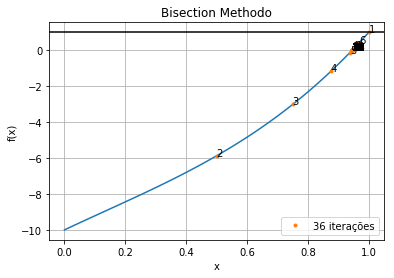
\includegraphics[scale=0.5]{/home/souza/Documents/semestre_2019-2/calculo_numerico/trabalho_1/graficos/bisection_f1.png}
    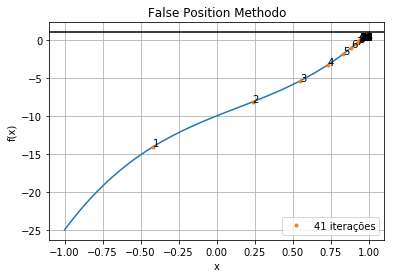
\includegraphics[scale=0.5]{/home/souza/Documents/semestre_2019-2/calculo_numerico/trabalho_1/graficos/false_position_f1.png}\\
    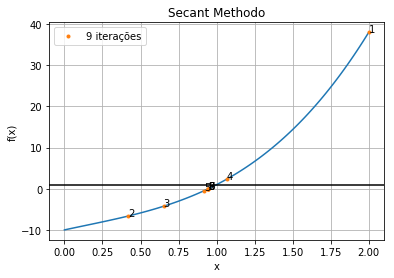
\includegraphics[scale=0.5]{/home/souza/Documents/semestre_2019-2/calculo_numerico/trabalho_1/graficos/secant_f1.png}
    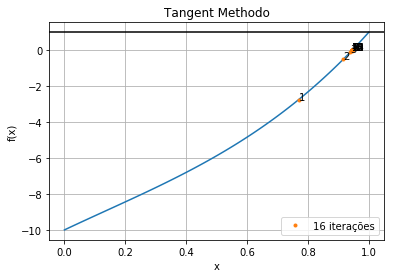
\includegraphics[scale=0.5]{/home/souza/Documents/semestre_2019-2/calculo_numerico/trabalho_1/graficos/tangent_f1.png}
    \caption{Gráficos da função um executada pelos quatro métodos presentes.}
\end{figure}

\begin{figure}[!ht]
    \centering
    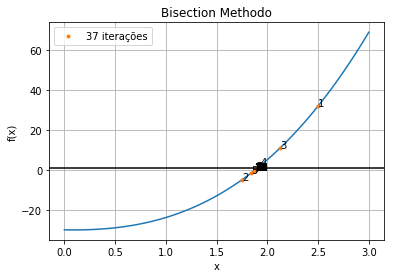
\includegraphics[scale=0.5]{/home/souza/Documents/semestre_2019-2/calculo_numerico/trabalho_1/graficos/bisection_f2.png}
    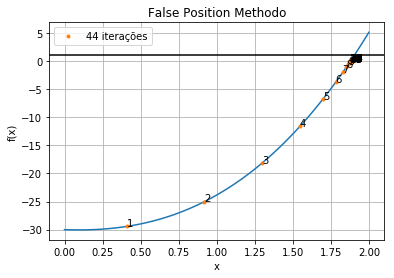
\includegraphics[scale=0.5]{/home/souza/Documents/semestre_2019-2/calculo_numerico/trabalho_1/graficos/false_position_f2.png}\\
    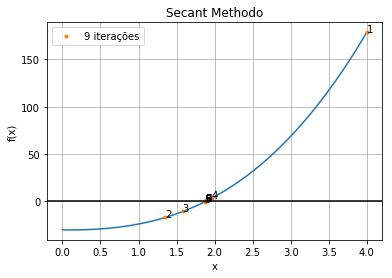
\includegraphics[scale=0.5]{/home/souza/Documents/semestre_2019-2/calculo_numerico/trabalho_1/graficos/secant_f2.png}
    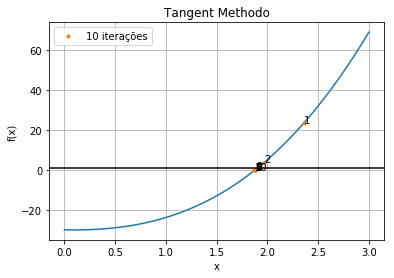
\includegraphics[scale=0.5]{/home/souza/Documents/semestre_2019-2/calculo_numerico/trabalho_1/graficos/tangent_f2.png}
    \caption{Gráficos da função dois executada pelos quatro métodos presentes.}
\end{figure}

\begin{figure}[!ht]
    \centering
    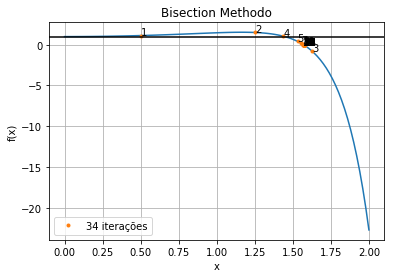
\includegraphics[scale=0.5]{/home/souza/Documents/semestre_2019-2/calculo_numerico/trabalho_1/graficos/bisection_f3.png}
    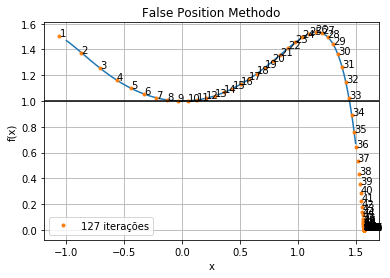
\includegraphics[scale=0.5]{/home/souza/Documents/semestre_2019-2/calculo_numerico/trabalho_1/graficos/false_position_f3.png}\\
    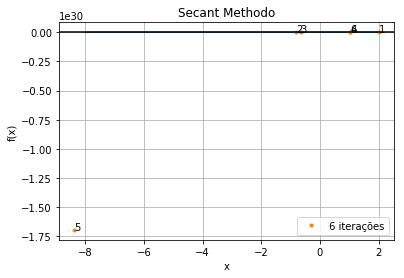
\includegraphics[scale=0.5]{/home/souza/Documents/semestre_2019-2/calculo_numerico/trabalho_1/graficos/secant_f3.png}
    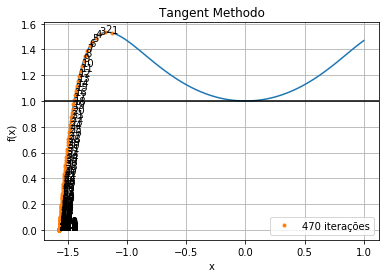
\includegraphics[scale=0.5]{/home/souza/Documents/semestre_2019-2/calculo_numerico/trabalho_1/graficos/tangent_f3.png}
    \caption{Gráficos da função três executada pelos quatro métodos presentes.}
\end{figure}

\begin{figure}[!ht]
    \centering
    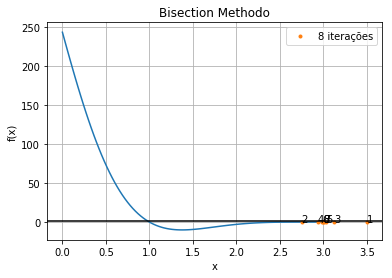
\includegraphics[scale=0.5]{/home/souza/Documents/semestre_2019-2/calculo_numerico/trabalho_1/graficos/bisection_f4.png}
    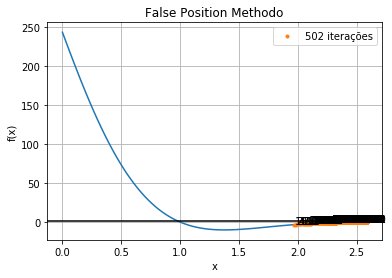
\includegraphics[scale=0.5]{/home/souza/Documents/semestre_2019-2/calculo_numerico/trabalho_1/graficos/false_position_f4.png}\\
    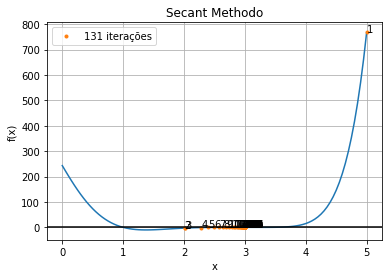
\includegraphics[scale=0.5]{/home/souza/Documents/semestre_2019-2/calculo_numerico/trabalho_1/graficos/secant_f4.png}
    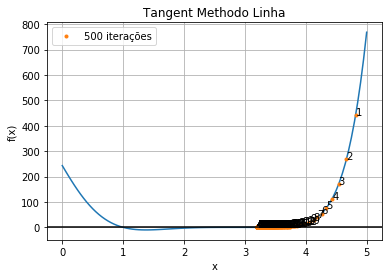
\includegraphics[scale=0.5]{/home/souza/Documents/semestre_2019-2/calculo_numerico/trabalho_1/graficos/tangent_f4.png}
    \caption{Gráficos da função quatro executada pelos quatro métodos presentes.}
\end{figure}

\begin{figure}[!ht]
    \centering
    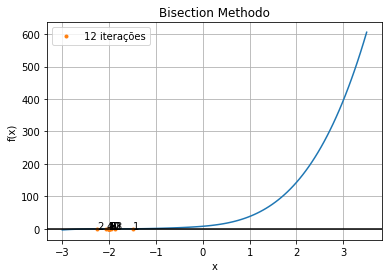
\includegraphics[scale=0.5]{/home/souza/Documents/semestre_2019-2/calculo_numerico/trabalho_1/graficos/bisection_f5.png}
    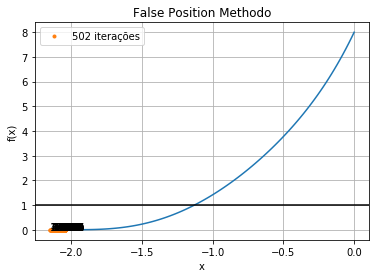
\includegraphics[scale=0.5]{/home/souza/Documents/semestre_2019-2/calculo_numerico/trabalho_1/graficos/false_position_f5.png}\\
    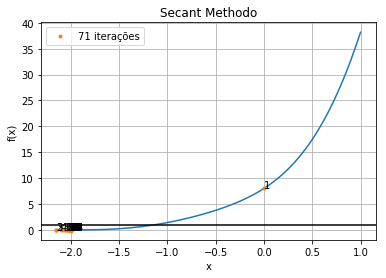
\includegraphics[scale=0.5]{/home/souza/Documents/semestre_2019-2/calculo_numerico/trabalho_1/graficos/secant_f5.png}
    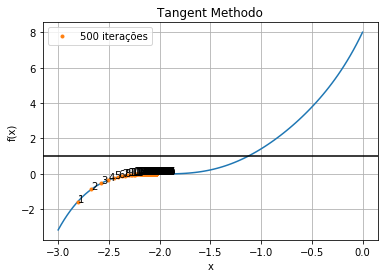
\includegraphics[scale=0.5]{/home/souza/Documents/semestre_2019-2/calculo_numerico/trabalho_1/graficos/tangent_f5.png}
    \caption{Gráficos da função cinco executada pelos quatro métodos presentes.}
\end{figure}
\end{document}
